In this chapter we introduce and clarify the technical concepts to necessary understand the later chapters. We also introduce the following notation that is used throughout the document:
\begin{itemize}
  \item Given a finite set $\cX$, let $\Delta(\cX)=\{p\in\real^\cX:\sum_x p(x)=1, p(x)\geq 0\;(\forall x)\}$ we denote the probability simplex on $\cX$. 
  \item Given a probability distribution $p\in\Delta(\cX)$, we let $\cB(p)=\{x\in\cX:p(x) > 0\}\subseteq\cX$ denote the support of $p$.
  \item Given a set $\cX$, let$\lvert\cX\rvert$ we denote the cardinality of set $\cX$.
  \item We use capital, non-caligraphic letters to express random variables while their lowercase counterpart represents a realization of such a random variable. E.g: $S_t$ is a random variable that denotes a state at timestep $t$ and $s_0$ is the realization of such random variable at timestep $0$.
\end{itemize}
\section{Markov decision processes}
Stochastic sequential decision problems in which a learning agent interacts sequentially with an environment are usually modeled as Markov decision processes (MDP). Without loss of generality, we restrict our attention to countable MDPs which are formally defined as the tuple $\cM=\langle\cS,\cA,\cR,\kernel,\kernel_0\rangle$, where:
\begin{itemize}
  \item $\cS$ is a countable set of states.
  \item $\cA$ is a finite set of actions.
  \item $\cR:\cS\times\cA\times\cS\rightarrow\real$ is a reward function. Though there exists multiple ways of defining a reward function (such as $\cR:\cS\times\cA\rightarrow\real$ or even $\linebreak\cR:\cS\rightarrow\real$), we stick to its most general form that associates rewards to triplets $\linebreak(s, a, s')\in\cS\times\cA\times\cS$. If necessary, we will redefine the reward functions accordingly.
  \item $\kernel:\cS\times\cA\rightarrow\Delta(\cS)$ is a transition probablity distribution that encondes $\kernel(\cdot\lvert s, a)$ for every $(s, a)\in\cS\times\cA$.
  \item $\kernel_0:\Delta(\cS)$ is the initial state distribution. We assume that $\kernel_0(s)>0\;\forall s\in\cS$.
\end{itemize}

The most general form of the interaction is depicted in Figure~\ref{fig:rl_loop}. At timestep $t$, the agent observes a state $S_t$ and chooses an action $A_t\sim\pi(S_t)$ according to a decision rule $\pi$. Such a decision rule is called the policy and it is a function 
\begin{equation}
\pi:\cS\rightarrow\Delta(\cA).
\label{eq:def_policy}
\end{equation}
This means the policy is a function that maps states to a distribution over actions. Once the agent executes action $A_t$ in the environment, it receives a reward $\linebreak R_{t+1} = \cR(S_t, A_t, S_{t+1})$ and a new state $S_{t+1}\sim\kernel(\cdot\lvert\cS_t, A_t)$. The process repeats indefinitely. Initially, the start state is sampled from the initial state distribution $S_0\sim\kernel_0$.

\begin{figure}
  \centering
  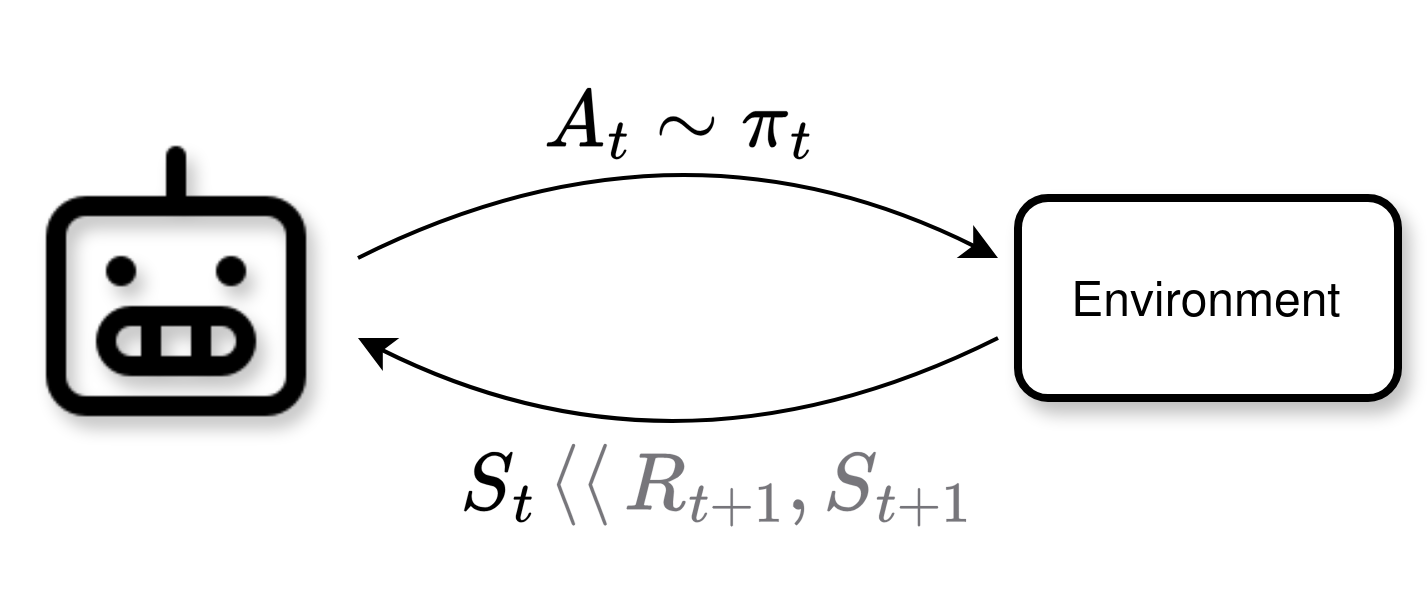
\includegraphics[width=0.65\textwidth]{figures/RL_loop.png}
  \caption{Interaction loop in a Markov decision process.}
  \label{fig:rl_loop}
\end{figure}


The quadruplet $(s_t, a_t, r_{t+1}, s_{t+1})$ defines a transition while the sequence of transitions up to a certain timestep, \[
  h_t = (s_0, s_0, r_1, s_1,\dots,r_t,s_t),
\] is called history. We let $\cH$ denote the set of all possible histories. Note that the interaction of an agent with the environment can be described by means of trajectories $h\in\cH$.

These processes are so-called Markov because the Markov property holds both in the reward and transition probability functions. This indicates that at timestep $t$ the reward and next state depends solely on the current state (or state and action), and not the full history. Formally this means that
\begin{align*}
  \kernel(s_{t+1}\lvert h_t) &= \kernel(s_{t+1}\lvert s_t, a_t), \\
  \cR(s_t, a_t, s_{t+1}\lvert h_t) &=  \cR(s_t, a_t, s_{t+1}) 
\end{align*}

There are many ways to design policies, but our definition in~\ref{eq:def_policy} implies that we will consider policies that:
\begin{itemize}
  \item are Markovian in the sense that the choice of the action depends on the current state $s_t\in\cS$ and not the whole trajectory $h_t\in\cH$, 
  \item are stationary, because they remain the same over time. To be more precise, the choice of the action given a state does not the depend on the timestep $t$ in which the state is observed,
  \item are stochastic as they represent a distribution over actions. More concretely a distribution $\pi(\cdot\lvert s)$ consitioned on the state $s\in\cS$. 
\end{itemize}
Unless otherwise specified, the policies considered satisfy the characteristics just mentioned. We will also need the notion of deterministic policies. In that case policies are functions $\pi:\cS\rightarrow\cA$ that return a single action for a given state, i.e~$a=\pi(s)$.


The aim of the learning agent is to come up with policies such that they optimize some numerical objective. Now, we turn our attention to two optimality cases: the discounted and the average-reward frameworks. In the following subsections we describe how we can solve each case when $\kernel$ and $\cR$ are fully disclosed to the agent via dynamic-programming. This setting, in which the reward and transition functions are known, is also referred to as planning in MDPs.


\subsection{The discounted case}
In the discounted setting, an optimal policy is such that it maximizes the expected discounted return. The discounted return is given by the sum of discounted rewards, 
\begin{equation}
  G_t = \sum_{i=t} ^\infty \gamma ^ {i-t} \cR(S_i, A_i, S_{i+1}).
  \label{eq:return}
\end{equation}
Here, $0<\gamma<1$ is the discount factor. There exists several reasons to use the discount factor, such as giving more credit to rewards closer in time. Notwithstanding, it is mainly used so as to make the return (Equation~\ref{eq:return}) have a finite value.

Given a policy $\pi$, we define its value function, $v^\pi:\cS\rightarrow\real$, as the expected discounted return of being at state $s\in\cS$ and following policy $\pi$,
\begin{equation}
  v^\pi(s) = \EEcp{\sum_{i=t} ^\infty \gamma ^ {i-t} R_i}{S_t = s}{\pi}\;\forall s\in\cS, 
\end{equation}
where $R_i$ is a shorthand for $\cR(S_i, A_i, S_{i+1})$. We also define the action-value function, $q^\pi:\cS\times\cA\rightarrow\real$, of a state-action pair as the expected discounted return of being at state $s\in\cS$, choosing action $a\in\cA$ and following policy $\pi$ thereafter,
\begin{equation}
  q^\pi(s, a) = \EEcp{\sum_{i=t} ^\infty \gamma ^ {i-t} R_i}{S_t = s, A_t = a}{\pi}\;\forall (s, a)\in\cS\times\cA.
\end{equation}
This value function is known to satisfy the following Bellman equations
\begin{equation}
  v^\pi(s) = \sum_a \pi(a\lvert s)\bigg[\sum_{s'} \cR(s, a, s') + \gamma \kernel(s'\lvert s, a)v^\pi(s')\bigg]\;\forall s\in\cS.
\end{equation}
Analogously, the action-value function satisfies the Bellman recursion given by 
\begin{equation}
  q^\pi(s, a) = \sum_{s'} \cR(s, a, s') + \gamma \kernel(s'\lvert s, a)v^\pi(s')\;\forall (s, a)\in\cS\times\cA.
\end{equation}
The goal of the agent is to compute a policy $\pi^*$ that maximizes the expected discounted return. We denote the optimal value and action-value functions attained by an optimal policy as $v^*$ and $q^*$, respectively. The question is how to obtain such optimal value functions so we can derive the optimal policy.

First, we describe how we can obtain the value function associated with a policy $\pi$. This procedure is usually known as policy evaluation. We declare the following Bellman operator $T^\pi:\real^\cS\rightarrow\real^\cS$ as 
\begin{equation}
  (T^\pi v^\pi)(s) = \sum_a \pi(a\lvert s)\bigg[\sum_{s'} \cR(s, a, s') + \gamma \kernel(s'\lvert s, a)v^\pi(s')\bigg]\;\forall s\in\cS.
  \label{eq:bo}
\end{equation}
By looking at $v^\pi$ as a vector of the appropiate size, Equation~\ref{eq:bo} can be rewritten in vector form as 
\begin{equation}
  T^\pi v^\pi = v^\pi.
\end{equation}
Therefore, computing the true value of $v^\pi$ requires finding the fixed-point solution of the previous system of linear equations. 

We further introduce the Bellman optimality operator $T^*:\real^\cS\rightarrow \real^\cS$ defined as
\begin{equation}
  (T^* v^*)(s) = \max_a \bigg[\sum_{s'} \cR(s, a, s') + \gamma \kernel(s'\lvert s, a)v^*(s')\bigg]\;\forall s\in\cS.
  \label{eq:boo}
\end{equation}
We can again rewrite~\ref{eq:boo} in vector form:
\begin{equation}
  T ^* v^* = v^*.
  \label{eq:boo_vector}
\end{equation}
The optimal value function $v^*$ is the fixed-point solution of the previous system of equations, which in this case is not linear as it requires a $\max$ operation. We can derive tge first dynamic-programming algorithm called value iteration from Equation~\ref{eq:boo_vector}. Here, we keep an estimate $v_k$ of the optimal value function function which updated iteratively as \[v_{k+1}\leftarrow T^* v_k,\] for some arbitrary initialization $v_0$. Value iteration can be shown to converge thanks to the contraction mapping theorem (see Appendix).

The idea of the operators can be also applied to the action-value function. Thus, we define the Bellman operator $T^\pi:\real^{\cS\times\cA}\rightarrow\real^{\cS\times\cA}$ and the Belmman optimality operator $T^*:\real^{\cS\times\cA}\rightarrow\real^{\cS\times\cA}$ over action-value functions in the following way:
\begin{align}
(T^\pi q^\pi)(s, a) &= \sum_{s'} \cR(s, a, s') + \gamma \kernel(s'\lvert s, a)v^\pi(s')\;\forall (s, a)\in\cS\times\cA. \\
(T^* q^*)(s, a) &= \sum_{s'} \cR(s, a, s') + \gamma \kernel(s'\lvert s, a)v^*(s')\;\forall (s, a)\in\cS\times\cA.
\end{align}
We also introduce the greedy operator $\cG:\real^{\cS}\rightarrow\cA^\cS$ over action-value functions which is defined as 
\begin{equation}
  (\cG q^\pi)(s, \cdot) = \argmax_a q^\pi(s, a) 
\end{equation}
and returns a deterministic, greedy policy with respect to the action-value function.
Now, we can describe the procedure called policy iteration, which consists of interleaved steps of policy evaluation and policy improvement operations. This algorithm works as follows
 \begin{enumerate}[label=(\arabic*)]
  \item Fix some initial policy $\pi_0$.
  \item At each iteration solve $T^{\pi_k} q^{\pi_k} = q^{\pi_k}$ (policy evaluation).
  \item Then derive new policy $\pi_{k+1}\leftarrow\cG q^{\pi_k}$ (policy improvement).
  \item Repeat (2) and (3) until convergence.
\end{enumerate}



\subsection{The average-reward case}
A better way to model continuing tasks is the average-reward setting. Here, the agent seeks a policy that maximizes 
\begin{equation}
  \rho^\pi(s) =\lim_{T\rightarrow\infty}\frac 1 T \mathbb{E}_\pi\left[\sum_{i=t}^T\cR(S_i, A_i, S_{i+1})\right] \;\forall s\in\cS
\end{equation}
which is known as the average-reward per step or gain.

This setting is arguably more complex than the discounted one and, usually, the following assumptions are made.

\begin{assumption}
  The MDP $\cM$ is communicating~\citep{Puterman1994}: for each pair of states $s,s'\in\cS$, there exists a policy $\pi$ that has non-zero probability of reaching $s'$ from $s$.
  \label{ass:mdp_communicating}
\end{assumption}

\begin{assumption}
  The ALMDP $\cM$ is unichain~\citep{Puterman1994}: the transition probability distribution induced by all stationary policies admit a single recurrent class.
  \label{ass:mdp_unichain}
\end{assumption}

In other words, we assume that$\dots$. A consquence of the aforeintroduced assumptions that simplify the analysis and algorithms is that the gain of any policy does not depend on the state, thus, $\rho^\pi(s) = \rho^\pi(s') = \rho^\pi = $. We use the latter term to denote the gain of a policy $\pi$.

Unlike the discounted case, the value functions could be now unbounded and, instead, relative value functions are used. are known to satisfy
\begin{align}
  v^\pi(s) &= \sum_a \pi(a\lvert s)\bigg[\sum_{s'} \cR(s, a, s') - \rho^\pi + \gamma \kernel(s'\lvert s, a)v^\pi(s')\bigg]\;\forall s\in\cS. \\
  q^\pi(s, a) &= \sum_{s'} \cR(s, a, s') - \rho^\pi + \gamma \kernel(s'\lvert s, a)v^\pi(s');\forall (s,a)\in\cS\times\cA. 
\end{align}

\section{Reinforcement learning}
When the agent is alien to the reward funtion $\cR$ and the transition function $\kernel$ of the MDP, the learning happens through direct interaction with the environment. Reinforcement learning (RL) proposes a learning paradigm in which the agent tries to learn the optimal behaviour by means of samples of that interaction. There is a vast collection of RL algorithms


\subsection{The discounted setting}
\subsection{The average-reward setting}

% \begin{figure}[t!h]
%     \centering
%     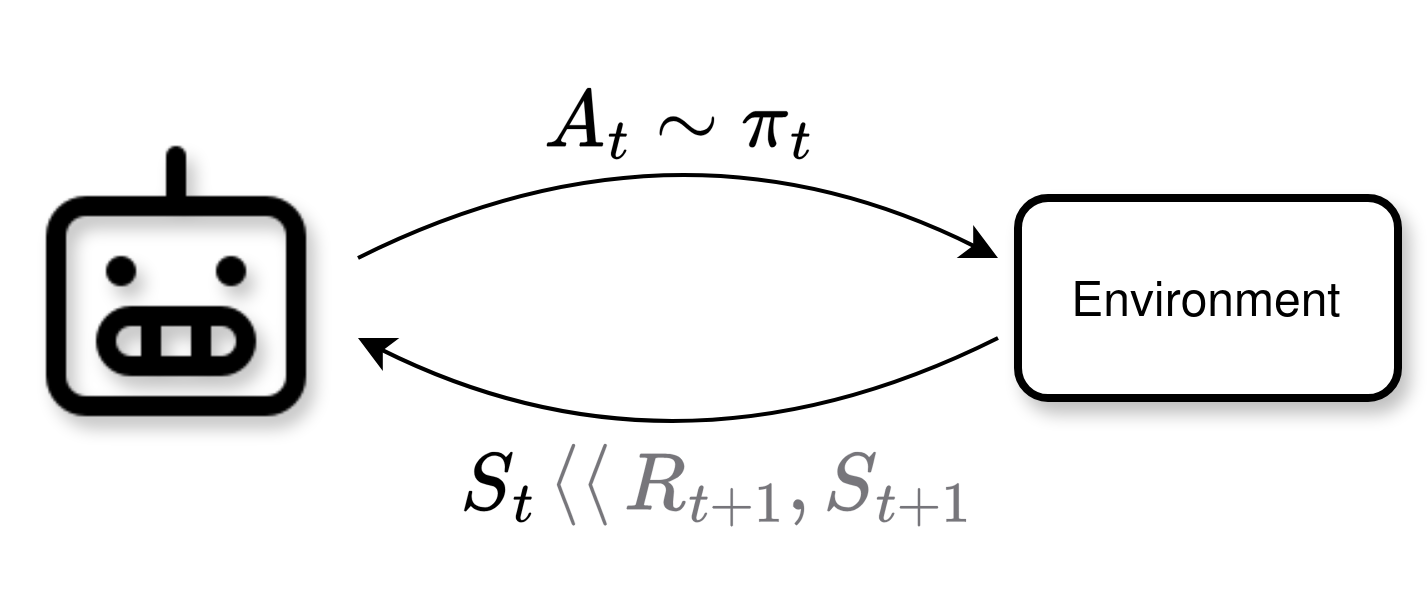
\includegraphics[width=0.65\textwidth]{figures/RL_loop.png}
%     \caption{Caption}
%     \label{fig:rl_loop}
% \end{figure}


\guillermo{
\section{Successor features} DEVELOP THIS FURTHER .. 

\label{section:successor_features}

Successor features (SFs)~\citep{Dayan1993, Barreto2017} is a widely used RL representation framework that assumes the reward function is linearly expressible with respect to a feature vector,
\begin{equation}
  \cR^\w(s, a, s') = \w^\intercal\boldsymbol\phi(s, a , s').
  \label{eq:reward_sf}
\end{equation}

Here, $\boldsymbol\phi:\cS\times\cA\times\cS\rightarrow\real^{d}$ maps transitions to feature vectors and $\w\in\real^d$ is a weight vector. Every weight vector~$\w$ induces a different reward function and, thus, a task. The SF vector of a state-action pair $(s,a)\in\cS\times\cA$ under a policy $\pi$ is the expected discounted sum of future feature vectors: 
\begin{equation}
  \boldpsi^\pi(s, a) = \EEcp{\sum_{i=t}^\infty \gamma^{i-t} \boldsymbol\phi_i}{S_t = s, A_t = a}{\pi},
  \label{eq:sf}
\end{equation}
where $\boldsymbol\phi_i = \boldsymbol\phi(S_{i}, A_{i}, S_{i+1})$. The action value function for a state-action pair $(s, a)$ under policy $\pi$ can be efficiently represented using the SF vector. Due to the linearity of the reward function, the weight vector can be decoupled from the Bellman recursion. Following the definition of Equations~\eqref{eq:qfunction}~ and \eqref{eq:reward_sf}, the action value function in the SF framework can be rewritten as
\begin{align}
  Q^\pi_\w(s, a) &= \EEcp{\sum_{i=t} ^\infty \gamma^{i-t} \w^\intercal\boldsymbol\phi_i}{S_t = s, A_t = a}{\pi} \nonumber \\
                 & = \w^\intercal\EEcp{\sum_{i=t} ^\infty \gamma^{i-t} \boldsymbol\phi_i}{S_t = s, A_t = a}{\pi} \nonumber \\
                 &=  \w^\intercal \boldpsi^\pi(s, a) .
\label{eq:qfunction_sf}
\end{align}

The SF representation leads to \textit{generalized policy evaluation} (GPE) over multiple tasks~\citep{Barreto2020a}, and similarly, to \textit{generalized policy improvement} (GPI) to obtain new better policies~\citep{Barreto2017}.

A family of MDPs is defined as the set of MDPs that share all the components, except the reward function. This set is formally defined as 
\begin{equation*}
    \cM^{\boldsymbol{\phi}}\equiv\{\langle\cS,\cE,\cA,\cR_\w,\mathbb{P}_0, \mathbb{P},\gamma\rangle \lvert \cR_\w = \w^\intercal \boldsymbol{\phi}, \forall\w\in\real^d\}.
\end{equation*}

Transfer learning on families of MDPs is possible thanks to GPI. Given a set of policies $\Pi$, learned on the same family~$\cM^{\boldsymbol{\phi}}$, for which their respective SF representations have been computed, and a new task $\w'\in\real^d$, a GPI policy $\pi_{\text{GPI}}$ for any $s\in\cS$ is derived as 
\begin{equation}
    \pi_{\text{GPI}}(s) \in \argmax_{a\in\cA} \max_{\pi\in\Pi} Q^\pi_{\w'}(s, a).
    \label{eq:gpi}
\end{equation}

However, there is no guarantee of optimality for $\w'$.
A fundamental question to solve the so-called \textit{optimal policy transfer learning problem} is which policies should be included in the set of policies $\Pi$ so an optimal policy for any weight vector $\w\in\real^d$ can be obtained with GPI. 
}

\section{Linearly-solvable Markov decision processes}

Linearly-solvable Markov decision processes~\citep{Todorov2006, Kappen2005} are a restricted class of the more general MDPs where the Bellman optimality equations are linear. This makes the computation of optimal value functions more efficient. In continuous state space domains or contexts of optimal control as probablistic inference, they frequently appear under the names of path-integral or Kullback-Leibler control~\citep{Kappen2012}. 

Even though this formulation is arguably restricted and only applicable to domains with deterministic dynamics, the intuition of entropy-regularization~\citep{Neu2017}, that lies at the core of LMDPs, is fundamental in RL as it is one of the building blocks of current state-of-the-art deep reinforcement learning algorithms such as trust region policy optimization~\citep{Schulman2015}, soft actor-critic (SAC)~\citep{Haarnoja2018} or Manchausen RL~\citep{Vieillard2020}. In what follows we introduce linearly-solvable Markov decision processes in the finite-horizon (first-exit) setting, its extension to infinite-horizon (average-reward) setting and we briefly discuss how they can be used along with function approximation.

\subsection{First-exit linearly-solvable Markov decision processes}

We define a first-exit linearly-solvable Markov decision process, or just LMDP, as a tuple $\cL=\langle\cS,\cT,\kernel,\cR,\cJ\rangle$, where: \begin{itemize}
  \item $\cS$ is a set of non-terminal states.
  \item $\cT$ is a set of terminal states.
  \item $\kernel:\cS\rightarrow\Delta(\cS^+)$ is an uncontrolled transition function, also known as passive dynamics or passive controls.
  \item $\cR:\cS\rightarrow\real$ is a reward function for non-terminal states.
  \item $\cJ:\cT\rightarrow\real$ is a reward function for terminal states.
\end{itemize}

\noindent We let $\cS^+=\cS\cup\cT$ denote the full set of states and $B=\max_{s\in\cS}|\cB(\kernel(\cdot|s))|$ an upper bound on the support of $\kernel$. 

Similarly to the stardard RL learning loop, the agent interacts with the environment in a sequential manner. Nontheless, there are no explict actions, and now the learning agent now follows a policy $\pi:\cS\rightarrow\Delta(\cS^+)$. Such a policy chooses, for each non-terminal state $s\in\cS$, a probability distribution over next states in the support of $\kernel(\cdot|s)$, i.e.~$\pi(\cdot|s)\in\Delta(\cB(\kernel(\cdot|s))$. There is also no explicit mention to the initial state distribution, which is asummed to be uniform over the set of non-terminal states (this is $\kernel_0 = \text{unif}(\cS)$). 

At each timestep $t$, the learning agent observes a state $s_t\in\cS^+$. If $s_t$ is non-terminal, the agent transitions to a new state $s_{t+1}\sim\pi(\cdot|s_t)$ and receives an immediate, regularized reward
\[
\cR(s_t, s_{t+1},\pi) = \cR(s_t) - \frac 1 \eta \log \frac {\pi(s_{t+1}|s_t)} {\kernel(s_{t+1}|s_t)},
\] 
where $\cR(s_t)$ is the reward associated with state $s_t$, and $\eta$ is a temperature parameter. 
%  $\mathrm{KL}(\pi(\cdot|s_t)\Vert\, \kernel(\cdot|s_t))$ is the Kullback-Leibler divergence between $\pi(\cdot|s_t)$ and $\kernel(\cdot|s_t)$ defined as 
% \begin{equation*}
%   \mathrm{KL}(\pi(\cdot|s)\Vert\, \kernel(\cdot|s)) = \sum_{s'} \pi(s'\lvert s) \log \frac{\pi(s'\lvert s)}{\kernel(s'\lvert s)}
% \end{equation*}

Hence the agent can set the probability $\pi(s_{t+1}|s_t)$ freely, but gets penalized by the entropy-regularization term for deviating from the passive controls $\kernel(s_{t+1}|s_t)$, and this penalty is modulated by the temperature parameter $\eta$. On the other hand, if $s_t$ is terminal, the agent receives reward $\cJ(s_t)$ and then the current episode ends. The aim of the agent is to compute a policy $\pi$ that maximizes the expected future \textbf{total reward}. For each non-terminal state $s\in\cS$, the value function is defined as
\[
v^\pi_\eta(s) = \EEc{\sum_{i=t}^{T-1} \cR(S_i, S_{i+1},\pi) + \cJ(S_T)}{S_t = s, \pi}.
\]

Here, $T$ is a random variable representing the time at which the current episode ends, and $S_t$ is a random variable representing the state at time $t$. The expectation is over the stochastic choice of next state $S_{t+1}\sim\pi(\cdot|S_t)$ at each time~$t$, and the time $T$ it takes for the episode to end. It is assumed that the reward of all non-terminal states is negative, i.e.~$\cR(s)<0$ for each $s\in\cS$. As a consequence, $\cR(s,\pi)<0$ holds for any policy $\pi$, and the value $v^\pi_\eta(s)$ has a well-defined upper bound. Note that the value function is computed with respect to a concrete value of the temperature parameter $\eta$.  
%As an alternative to the assumption $\cR(s)<0$, we could instead assume that each policy terminates with probability 1 within a fixed time horizon $H$.


We are interested in finding the optimal policy which implies computing the optimal value function ${v^*_\eta:\cS\rightarrow\real}$, i.e.~the maximum expected future total reward among all policies. The value function is extended to each terminal state $\tau\in\cT$ by defining $v^*_\eta(\tau)\equiv\eta\cJ(\tau)$. The value function $v^*_\eta$ satisfies the Bellman equations
\begin{align*}
  \eta v^*_\eta(s) &= \eta \max_\pi \left[ \cR(s,\pi) + \mathbb{E}_{s'\sim\pi(\cdot|s)} v^*_\eta(s') \right] \\
  &= \eta \cR(s) + \max_\pi \mathbb{E}_{s'\sim\pi(\cdot|s)} \left[ \eta v^*_\eta(s') - \log \frac {\pi(s'|s)} {\kernel(s'|s)} \right] \;\; \forall s.
\end{align*}
In expectation, the regularization term in reduces to the Kullback-Liebler divergence between $\pi$ and $\kernel$,
\begin{equation*}
  \mathbb{E}_{s'\sim\pi(\cdot|s)} \log \frac {\pi(s'|s)} {\kernel(s'|s)} = \sum_{s'}\kernel(s'\lvert s)\log\frac{\pi(s'\lvert s)}{\kernel(s'\lvert s)} = \mathrm{KL}\big(\pi(\cdot|s)\Vert\, \kernel(\cdot|s)\big).
\end{equation*}

The maximization in the Bellman equations can be resolved analytically~\citep{Todorov2006}, and the optimal value function can be rewritten as
\begin{align*}
  v^*_\eta(s)      &=  \frac 1 \eta \log{\sum_{s'\in\cS}\kernel(s'\lvert s)e^{\eta(\cR(s) + v^*_\eta(s'))})} \;\;\forall s\in\cS, \\
                   &=  \cR(s) + \frac 1 \eta \log{\sum_{s'\in\cS}\kernel(s'\lvert s)e^{\eta v^*_\eta(s')}} \;\;\forall s\in\cS, \\
  \eta v^*_\eta(s) &=  \eta \cR(s) + \log{\sum_{s'\in\cS}\kernel(s'\lvert s)e^{\eta v^*_\eta(s')}} \;\;\forall s\in\cS.
\end{align*}
Now, we introduce the notation $z(s)=e^{\eta v^*_\eta(s)}$ for each $s\in\cS^+$. We often abuse this notation by referring to $z(s)$ as the (optimal) value of $s$. After exponentiating, the previous system yields the following Bellman optimality equations that are linear in $z$:
\begin{equation}\label{eq:boe_z_lmdp}
z(s) = e^{\eta\cR(s)} \sum_{s'}\kernel(s'|s)z(s').
\end{equation}
\subsubsection{Solving a first-exit LMDP}
The Bellman equation can be expressed in matrix form by defining an $\lvert\cS\rvert\times\lvert\cS\rvert$ diagonal reward matrix $R=\diag(e^{\eta\cR(\cdot)})$ and an $\lvert\cS\rvert\times \lvert\cS^+\rvert$ stochastic transition matrix $P$ whose entries $(s,s')$ equal $\kernel(s'|s)$. We define a vector $\bf z$ that stores the values $z(s)$ for each non-terminal state $s\in\cS$, and a vector $\bf z^+$ extended to all states in $\cS^+$. Now we can write the Bellman equations in matrix form as:
\begin{equation}\label{eq:eigen_lmdp}
{\bf z} = R P {\bf z^+}.
\end{equation}
Given $z$, the optimal policy $\pi$ is given by the following expression for each pair of states $(s,s')$:
\begin{equation}
\label{eq:lmdp_optimal_policy}
\pi(s'|s) =  \frac {\kernel(s'|s) e^{\eta v(s')} } {\sum_{s''} \kernel(s''|s) e^{\eta v(s'')} } = \frac {\kernel(s'|s)z(s')} {\sum_{s''} \kernel(s''|s)z(s'')}.
\end{equation}

The solution for $z$ corresponds to the largest eigenvector of $RP$.
If the dynamics $\kernel$ and $\cR$ are known, we can iterate~\eqref{eq:eigen_lmdp}~\citep{Todorov2006}.

Alternatively, we can learn an estimate $\widehat{z}$ incrementally using stochastic updates based on state transitions sampled from the uncontrolled dynamics $(s_t,r_t,s_{t+1})$
% use an online algorithm called Z-learning to compute an estimate  \citep{TodorovNIPS2007}. After observing each transition , the update rule of Z-learning is given by
\[
\widehat{z}(s_t) \leftarrow (1-\alpha_t)\widehat{z}(s_t) + \alpha_t e^{\eta r_t}\widehat{z}(s_{t+1}),
\]
where $\alpha_t$ is a learning rate. 
The previous update rule is called \emph{Z-learning}~\citep{Todorov2006} and suffers from slow convergence in very large state spaces and when the optimal policy differs substantially from the uncontrolled dynamics $\kernel$.
%assumes that we sample next states using the uncontrolled transition function $\cP$, which is typically no better than a random walk. 
A better choice is importance sampling, which uses samples from the estimated policy $\widehat{\pi}$ derived from the estimated values $\widehat{z}$ and \eqref{eq:lmdp_optimal_policy} and updates $\widehat{z}$ according to the following update
%to obtain samples that are corrected using the following update~\citet{TodorovPNAS2009}:
%to sample In this case,  suggested a corrected update rule based on importance sampling:
\begin{align}\label{eqn:zlearning-imp}
\widehat{z}(s_t) \leftarrow (1-\alpha_t)& \widehat{z}(s_t) + \alpha_t e^{\eta r_t}\widehat{z}(s_{t+1})\frac {\kernel(s_{t+1}|s_t)} {\widehat{\pi}(s_{t+1}|s_t)}.
\end{align}
However, this requires local knowledge of $\kernel(\cdot|s_t)$ to correct for the different sampling distribution.
%, i.e.~the set of possible next states and their associated uncontrolled probabilities.
Though this seems like a strong assumption, in practice $\kernel$ usually has a simple form, e.g.~uniform distribution.
Further, as shown in \citep{Jonsson2016}, the corrected update rule in \eqref{eqn:zlearning-imp} can also be used to perform off-policy updates in case transitions are sampled using a policy different from $\widehat{\pi}$.
%leading to simultaneous learning of different tasks.
%Note that the expression for the policy $\widehat{\pi}$ in \eqref{eq:pi} and the corrected update rule in \eqref{eqn:zlearning-imp} require local knowledge of $\cP(\cdot|s_t)$, i.e.~the set of possible next states and their associated uncontrolled probabilities. Though this seems like a strong assumption, in practice $\cP$ usually has a simple form, e.g.~uniform. \citet{conf/icaps/Jonsson16} showed that the corrected update rule in \eqref{eqn:zlearning-imp} can also be used to perform off-policy updates in case transitions are sampled using a policy different from $\widehat{\pi}$.

\subsubsection{Compositionality}
\label{section:compositionality}
\citet{Todorov2009a} introduces the concept of compositionality for LMDPs. Let us consider a set of LMDPs $\{\cL_1,\ldots,\cL_n\}$, where each LMDP $\cL_i=\langle\cS,\cT,\kernel,\cR,\cJ_i\rangle$ has the same components $\cS,\cT,\kernel,\cR$ and only differ in the reward $\cJ_i(\tau)$ of each terminal state $\tau\in\cT$, as well as its exponentiated value $z_i(\tau)=e^{\eta \cJ_i(\tau)}$.

Now consider a new LMDP $\cL=\langle\cS,\cT,\kernel,\cR,\cJ\rangle$ with the same components as the $n$ LMDPs above, except for $\cJ$. Assume that there exist weights $w_1,\ldots,w_n$ such that the exponentiated value of each terminal state $\tau\in\cT$ can be written as
\[
e^{\eta \cJ(\tau)} = z(\tau) = w_1z_1(\tau) + \ldots + w_nz_n(\tau) = \sum_{k=1}^n w_kz_k(\tau).
\]
Since the Bellman optimality equation of each non-terminal state $s\in\cS$ is linear in $z$, the optimal value of $s$ satisfies the same equation:
\[
z(s) = \sum_{k=1}^n w_kz_k(s).
\]
Consequently, if the optimal values $z_1,\ldots,z_n$ of the $n$ LMDPs are previously computed and the weights $w_1,\ldots,w_n$ are known, we immediately obtains the optimal values of the new LMDP $\cL$ without further learning.


\subsection{Average-reward linearly-solvable Markov decision processes}

LMDPs can be extended to the average-reward setting. We say an average-reward Linearly-solvable Markov decision process (ALMDP) is a tuple
$\cL = \langle\cS,\kernel,\cR\rangle$, where $\cS$ is a set of states, $\kernel:\cS\rightarrow\Delta(\cS)$ is the passive dynamics, and $\cR$ is the reward function. ALMDPs represent infinite-horizon (continuing) tasks and, unlike first-exit LMDPs, there are no terminal states. Consequently, there is no reward function for terminal states.  

Throughout this thesis, we make the following assumptions about ALMDPs. These are common assumptions in the average-reward RL setting to avoid ill-defined value functions.

\begin{assumption}
  The ALMDP $\cL$ is communicating~\citep{Puterman1994}: for each pair of states $s,s'\in\cS$, there exists a policy $\pi$ that has non-zero probability of reaching $s'$ from $s$.
  \label{ass:communicating}
\end{assumption}

\begin{assumption}
  The ALMDP $\cL$ is unichain~\citep{Puterman1994}: the transition probability distribution induced by all stationary policies admit a single recurrent class.
  \label{ass:unichain}
\end{assumption}
%\todo{I think this assumption is enough: no need to introduce the notation for stationary distributions over the state space since we do not use it at any point. This assumption as is is enough to make the gain not to be conditioned by the initial state.}
%{\color{red} \begin{assumption}
%  For all states $s\in\cS$ the reward $\cR(s)$ is bounded in $\left(-\infty, 0\right]$.
%  \label{ass:rewards}
%\end{assumption}}

In the average-reward setting, the value function is defined as the expected \textbf{average reward} when following a policy $\pi:\cS\rightarrow\Delta(\cS)$ starting from a state $s\in\cS$. This is expressed as
\begin{equation}
  v_\eta^\pi(s) = \underset{T\rightarrow\infty}\lim \EEc{\frac{1}{T} \sum_{i=t}^T \cR(S_i, S_{i+1}, \pi)}{S_t = s, \pi},
  \label{eq:value_function_almdp}
\end{equation}
where $\cR(s_t, s_{t+1}, \pi)$ is defined as for first-exit LMDPs.
Again, the goal is to obtain the optimal value function $v^*_\eta$. Under Assumption~\ref{ass:unichain}, the Bellman optimality equations can be written as
\begin{equation}
  v^*_\eta(s) = \frac 1 \eta \log{\sum_{s'\in\cS}\kernel(s'\lvert s)e^{\eta(\cR(s) - \rho + v^*_\eta(s'))}} \;\;\forall s\in\cS,
  \label{eq:boe_almdp}
\end{equation}
where $\rho$ is the optimal one-step average reward (i.e.~gain), which is state-independent for unichain\todo{Add derivation of the independece of the gain?} ALMDPs~\citep{Todorov2006}. Exponentiating yields
\begin{equation}
  z(s) = e^{\eta(\cR(s) - \rho)} \sum_{s'\in\cS}\kernel(s'\lvert s)z(s') \;\;\forall s\in\cS.
  \label{eq:boe_z_almdp}
\end{equation}
For the optimal value function $z$, the optimal policy is given by the same expression as in~\eqref{eq:lmdp_optimal_policy}.

\subsubsection{Solving an ALMDP}

We let $\Gamma=e^{\eta\rho}$ denote the exponentiated gain. Similar to the first-exit case, we can express Equation~\eqref{eq:boe_z_almdp} in matrix form as
\begin{equation}\label{eq:rel_opt}
  \Gamma {\bf z} = R P {\bf z},
\end{equation}
where the matrices $P\in \real^{\lvert\cS\rvert\times\lvert\cS\rvert}$ and $R\in \real^{\lvert\cS\rvert\times\lvert\cS\rvert}$ are appropiately defined as in~\eqref{eq:eigen_lmdp}. The exponentiated gain $\Gamma$ can be shown to correspond to the largest eigenvalue of $RP$~\citep{Todorov2009}.
An ALMDP can be solved using {\em relative value iteration} by selecting a reference state $s^*\in\cS$, initializing $\widehat{\bf z}_0={\bf 1}$ and iteratively applying
\begin{equation*}
  \widehat{\bf z}_{k+\frac 1 2} \gets R P \widehat{\bf z}_k, \quad \quad \widehat{\bf z}_{k+1} \gets \widehat{\bf z}_{k+\frac 1 2} / \widehat z_{k+\frac 1 2}(s^*).
\end{equation*}
The reference state $s^*$ satisfies $z(s^*)=1$, which makes the optimal value $z$ unique (else any constant shift preserves optimality). After convergence, the exponentiated gain equals $\Gamma=\widehat z_{k+\frac 1 2}(s^*)$. Under Assumption~\ref{ass:communicating}, relative value iteration converges to the unique optimal value $z$~\citep{Todorov2009}.

Analogously to first-exit LMDPs, when $\kernel$ and $\cR$ are not known, the agent can learn estimates $\widehat z$ and $\widehat\Gamma$ of the optimal value function and the exponentiated gain in an online manner, using samples $(s_t, r_t, s_{t+1})$ generated when following the estimated policy $\widehat\pi$. The update rules for the so-called \textit{differential Z-learning} algorithm are given by
\begin{align}
  \widehat{z}_{t+1}(s_t)  \gets \widehat{z}_{t}(s_{t}) & + \alpha_t \Bigg(\frac{e^{\eta r_t}}{\widehat\Gamma_t}\dfrac{\kernel(s_{t+1}\lvert s_t)}{\widehat\pi_t(s_{t+1}\lvert s_t)}  - \widehat z_t(s_t)\Bigg),\label{eq:diff_update_z}  \\   %\delta^z_t \\
  \widehat\Gamma_{t+1}    \gets \widehat\Gamma_t       & + \beta_t \Bigg(\frac{e^{\eta r_t}}{\widehat z_t(s_t)}\dfrac{\kernel(s_{t+1}\lvert s_t)}{\widehat\pi_t(s_{t+1}\lvert s_t)}  - \widehat \Gamma_t\Bigg).\label{eq:diff_update_gamma}
\end{align}
The learning rates $\alpha_t$ and $\beta_t$ can be chosen independently.

Unlike the first-exit case, the compositionality property does not hold in the average-reward case.

\subsection{Function approximation in LMDPs}

So far, we have introduced methods for solving (A)LMDPs in the tabular case, where the full state space can be enumerated and stored in memory. However, in cases where the state space is considerably large, tabular methods are unfeasible and the value function is approximated.

In this line,~\cite{Todorov2010} prescibes two families of methods for adapting LMDPs in the average-reward setting to function approximation. The first one lies in the family of policy gradients while the second ones can be considered critic-only approaches. Here a valid parameterization of the policy $\pi(s'\lvert s, \w)$ is considered.

The Bellman equation~\eqref{eq:boe_almdp} can be rewritten as follows
\begin{equation}
\label{eq:boe_for_pg}
\rho + v^*(s) =\cR(s) +\log{\sum_{s'\in\cS}\kernel(s'\lvert s)e^{v^*(s')}} \;\;\forall s\in\cS,
\end{equation}
for the sake of simplicity we assume that $\eta=1$. 

The first flavor of methods builds on the policy gradient theorem for ALMDPs~\citep[cf.~Theorem 1]{Todorov2010} that states that the gradient of the gain in ALMDPs is
\begin{equation}
  \nabla_\w \rho = \sum_{s}\mu(s, \w) \sum_{s'} \nabla_\w \pi(s'\lvert s, \w)\Big( \log \frac{\pi(s'\lvert s, \w)}{\kernel(s'\lvert s)} + \widetilde v(s', \mathbf{r})\Big),
\end{equation}
where $\mu(x, \w)$ is the stationary distribution induced by $\pi$, and $\widetilde v(s,\mathbf{r})$ is an approximation to the (optimal) value function with parameterization $\mathbf r$.

For the second type of methods one could use \textit{approximate} value iteration or \textit{approximate} policy iteration to iteratively improve the weight vector $\w$, even though this results in a biased estimator. An even more direct approach is to use Gauss-Newton method to fit the weight vector $\w$ by directly optimizing~\eqref{eq:boe_for_pg}.

Despite the correctness of the theoretical results, which guarantee that function approximation can be used along with LMDPs, they are of little practical use. Even in the linear function approximation (LFA) case, obtaining a correct parameterization for $\widetilde v(s,\mathbf{r})$ requires of an intricate process in the policy gradient approach. Additionally, the representation of the policy still depends on the size of the whole state space. This makes the approach intractable for real-world problems as it does not scale with large state spaces.


\section{Hierarchical Reinforcement Learning}
Hierarchical Reinforcement learning embodies the idea of divide-and-conquer in sequential decision problems. 
\subsection{Optimality of HRL algorithms}
\cite{Dietterich2000} identifies two types of optimality for hierarchical methods in reinforcement learning, namely \textit{hierarchical optimality} and \textit{recursive optimality}. Hierarchical optimality implies optimality with regard a constrained space of policies, given by the hierarchy structure. Hierarchies of Abtract Machines (HAMs,~\cite{Parr1997}) and the Options Framework~\citep{Sutton1999} lie in this category) 
\subsection{The options framework}
\label{section:options}

\section{Non-Markovian task specification}
\label{section:non_markovian}
 {\color{blue}
 
 \begin{itemize}
 \item Difficulty about expressing some tasks in Marokovian terms 
 \item Finite State Autamatons and Reward Machines 
 \item Reward Machines and their relationship with logics
 \item Comment on algorithms given in the 
  
\end{itemize}
 
 }


